\documentclass[journal, a4paper]{IEEEtran}

\usepackage{graphicx}   
%\usepackage{subfigure}
\usepackage{url}        
\usepackage{amsmath}    
% Some useful/example abbreviations for writing math
\newcommand{\argmax}{\operatornamewithlimits{argmax}}
\newcommand{\argmin}{\operatornamewithlimits{argmin}}
\newcommand{\x}{\mathbf{x}}
\newcommand{\y}{\mathbf{y}}
\newcommand{\ypred}{\mathbf{\hat y}}

% Start of added stuff by lukas
%\newtheorem{defi}{Definition}[section]
% Packages
\usepackage{mathtools}
\usepackage{amsmath}
\usepackage{amssymb}
\usepackage{amsthm}
% Theorems and definitions
\theoremstyle{plain}
\newtheorem{thm}{Theorem}[section]
\theoremstyle{definition}
\newtheorem{defn}[thm]{Definition}
% End of added stuff by lukas

\begin{document}

% Define document title, do NOT write author names
\title{The Title of your Report}
\author{Anonymous Authors}
\maketitle

% Write abstract here
\begin{abstract}
	A short summary of your project. You should change also the title, but do \emph{not} enter any author names or anything that unnecessarily identifies any of the authors. It is suggested you use a similar structure (sections, etc.) as demonstrated in this document, but you can make the section headings more descriptive if you wish. Of course \emph{you should delete all the text in this template and write your own}! -- this text simply provides detailed instructions/hints on how to proceed.

\end{abstract}

% Each section begins with a \section{title} command
\section{Introduction}

Describe what you did. Provide access to your anonymized code\footnote{Our code is available here: \url{http://anonymouslinktoyourcode.zip}}.

Note that results should be reproducible using the technologies from the labs (i.e., Python, and selecting among Scikit-Learn, OpenAI Gym, TensorFlow, PyGame, \ldots).

Do not change the formatting (columns, margins, etc). Hint: shared tools like \texttt{http://sharelatex.com/} and \texttt{http://overleaf.com/} are great tools for collaborating on a multi-author report in latex. If you wish to use Word, base it on the IEEE template\footnote{\url{https://www.ieee.org/publications_standards/publications/conferences/2014_04_msw_a4_format.doc}} and convert to \texttt{pdf} for submission. 

\section{Background and Related Work}

Elaborate (in your own words) the background material required to understand your work. It should cover a subset of the topics touched upon in the course. You are encouraged to cite topics in lectures, e.g., structured output prediction in \cite{LectureSOP}, book chapters, e.g., Chapter 9 from \cite{Barber}, or articles from the literature, e.g., \cite{Astar,DeepMindSC2}. Basically, you should prepare the reader to understand what you are about to present in the following sections. Eq.~\eqref{eq:MAP} shows a random equation.
\begin{equation}
	\label{eq:MAP}
	% Note the example \newcommand s defined above which make it faster to write latex math
	\ypred = \argmax_{\y \in \{0,1\}} p(\y|\x)
\end{equation}

\section{The Environment}
In this report we work with a supply-chain optimization environment over an infinite amount of periods. The environment consists of one factory and up to $k \in \mathbb{N}$ warehouses where in each period it needs to be decided how many units of a product (e.g. butter) should be produced and how many should be shipped to the individual warehouses. A representation of a network with 5 warehouses is depicted in figure \ref{fig:model_example}. 
\begin{figure}[h]
	\label{fig:model_example}
	\centering
	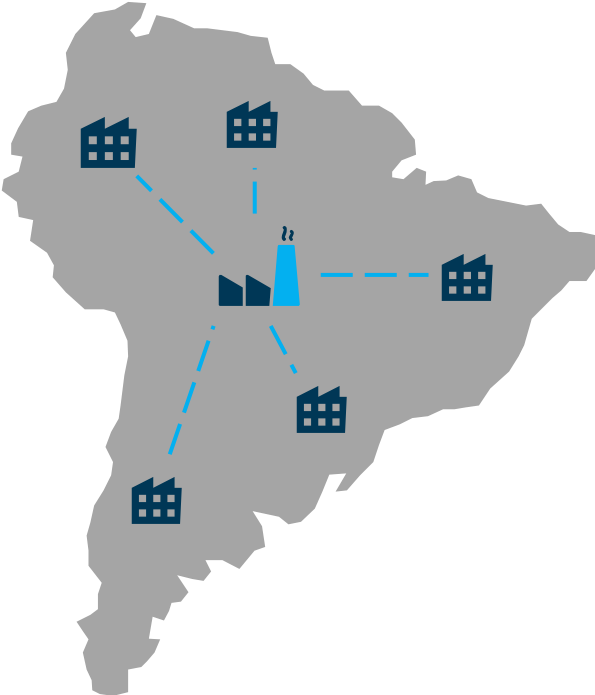
\includegraphics[width=0.4\columnwidth]{model.png}
	\caption{\label{a_figure}Example of a supply chain network with $k=5$ warehouses ($s_1, .., s_5$) the factory ($s_0$).}
\end{figure}
The state space consists of $k+1$ elements describing the current stock level of the factory / the warehouses where each stock level is limited by some $c_j \in \mathbb{N}$. Furthermore we include an environment process $D$ describing the (stochastic) demand $d_j$ at each warehouse $j = 1,...,k$. In each period the agent can now set the production level for the next period $a_0 \in \{0,.., \rho_{max}\}$ where $\rho_{max} \in \mathbb{N}$ is the maximum production aswell as the amount of products that is shipped to each location $a_j \in \mathbb{N}^k$ that is naturally limited by the current storage level in the factory ($\sum_{j=1}^{k}a_j \leq s_0$). Based on this information and the demand $d$ we can now describe the transition for $s_0$, $s_j, \ j = 1,..., k$ by
\begin{equation}
	\begin{split}
		s_0' = &\min\{s_0 + a_0 - \sum_{j=1}^{k}a_j \}, \\
		s_j' = &\min\{s_j + a_j - d_j\}, \ j=1,...,k.
	\end{split}
	\end{equation}
The reward within each period consists of the revenue from sold products at a fix price $p$ less production costs $\kappa_{pr}a_0$, storage costs $\sum_{j=0}^{k}\kappa_{st,j} \max\{s_j, 0\}$, penalty costs $\kappa_{pe} \sum_{j=1}^{k}\min\{s_j,0\}$ and transportation costs $\sum_{j=1}^{k} \kappa_{tr, j} \left\lceil a_j / \zeta_j \right\rceil$. We let $p, \kappa_{pr}, \kappa_{pe}, \kappa_{st, j}, \kappa_{tr,j} \in \mathbb{R}$ and $\zeta_j \in \mathbb{N}$ for $i=1,...,k$. We can now define the one-step reward function by
\begin{equation}
\label{eq:one_ste_reward}
	\begin{split}
		r(s, d, a) \coloneqq &p \sum_{j=1}^{k}d_i - \kappa_{pr} a_0 - \sum_{j=0}^{k} \kappa_{st, j} \max\{s_j, 0\} \\ 
		&-\kappa_{pe} \sum_{j=1}^{k}\min\{s_j, 0\} - \sum_{j=1}^{k} \kappa_{tr, j} \left\lceil \frac{a_j}{\zeta_j} \right\rceil
	\end{split}
\end{equation}
with $\left\lceil x \right\rceil$ the ceiling of $x$. Based on the model description we can now formulate the task as an infinite horizon markov decision process that is subject to a varying environment. Thereby we receive the tuple $(S, D, A, \mathcal{X}, T, Q, r, \gamma)$ with
\begin{defn} \label{def:modell} \
	\begin{itemize}
		\item[1.] $S \times D \coloneqq \prod\limits_{j=0}^{k} \{s_j \in \mathbb{Z} \ | \ s_j \leq c_j\} \times D, c_j \in \mathbb{N}$ the state space consisting of elements $(s,d) = ((s_0, s_1, ... , s_k), d)$;
		\item[2.] $ A \coloneqq  \{0, ..., \rho_{max} \} \times \mathbb{N}_0^k$ the action space consisting of elements $a = (a_0, ..., a_k)$;
		\item[3.] $ \mathcal{X} (s) \coloneqq \{0, ..., \rho_{max} \} \times \{a \in \mathbb{N}_0^k \ | \ \sum_{j=1}^{k}a_j \leq s_0  \}$, the set of all feasible actions in a state $s$ and $\mathcal{X} \coloneqq \{(s, d , a) \in S \times D \times A \ | \ a \in \mathcal{X} (s)\}$;
		\item[4.] $ T: S \times D \times A \rightarrow S$ the transition function defined by
			\begin{equation*}
				\begin{split}
					T(s, d, a) \coloneqq &(\min\{s_0 + a_0 - \sum_{j=1}^{k}a_j, c_0 \}, \\
					&\min\{s_1 + a_1 - d_1, c_1 \}, \\
					&\ ... \\
					&\min\{s_k + a_k - d_k, c_k \});
				\end{split}
			\end{equation*}
		\item[5.] $ Q: \mathcal{X} \times S \times D \rightarrow [0,1]  $ the transition probabilities defined by $Q(s', d'\ |\ s, d, a) \coloneqq q_d(d')$ for $s' = T(s, d, a)$ and $0$ otherwise;
		\item[6.] $ r: S \times D \times A \rightarrow \mathbb{R} $ the one-step reward function as defined in Eq.~\eqref{eq:one_ste_reward};
%			\begin{equation*}
%				\begin{split}
%					r(s, d, a) \coloneqq &p \sum_{j=1}^{k}d_i - \kappa_{pr} a_0 - \sum_{j=0}^{k} \kappa_{st, j} \max\{s_j, 0\} \\ 
%					&-\kappa_{pe} \sum_{j=1}^{k}\min\{s_j, 0\} - \sum_{j=1}^{k} \kappa_{tr, j} \left\lceil \frac{a_j}{\zeta_j} \right\rceil;
%				\end{split}
%			\end{equation*}
		\item[7.] $\gamma \in (0, 1) $ the discounting factor.
	\end{itemize}
\end{defn}
For the calculation of the expected discounted revenue for each tuple $(s, d)$ we obtain the value function $V$ with\\
\begin{equation}
	\label{eq:ValueFunction}
	\begin{split}
		V(s,d) = &\max_{a \in \mathcal{X} (s)} \{ r(s, d, a)  \\
		&+ \gamma \sum_{d' \in D} q_d(d') V(T(s, d, a), d') \}, \\ 
		&s \in S, d \in D. 
	\end{split}
\end{equation}
\section{The Agent}

The agent you designed for your environment. Justify your choice and design and explain briefly how you implemented/configured it. Naturally, if you took a ready-made environment, you should invert relatively much more effort into this section than the previous one.

\section{Results and Discussion}

This is one of the most important sections. You put your agent to the test in the environment, you show -- and most importantly -- you interpret the results.

\subsection{Performance of your Agent in your Environment}

Show plots, graphs, tables (e.g., Table~\ref{a_table}), etc. You may wish to encourage readers to reproduce results for themselves, e.g., run \texttt{runDemo.py} in our source code. Show how your agent performs well, or, if it doesn't perform well, it is better to explain why (this is a result in itself!). In any case, you \emph{must} highlight the weaknesses of your agent as well as its strengths.

\begin{table}[h]
	\caption{\label{a_table}This table is just an example.}
	\centering
	\begin{tabular}{lll}
		\hline
		\textbf{Environment config.} & \textbf{Standard SARSA} & \textbf{Our Improved Agent}  \\
		\hline
		Simulation 1        & 10             & 15 \\
		Simulation 2        & 12             & 11 \\
		\hline
	\end{tabular}
\end{table}

\subsection{Performance of your Agent in the ALife Environment}

You deploy your agent in the ALife\footnote{\url{https://github.com/jmread/alife}} environment (a random screenshot shown in Figure~\ref{a_figure}). Does it work well? Why? Why not? Justify the adaptation you think is best.

\begin{figure}[h]
	\centering
	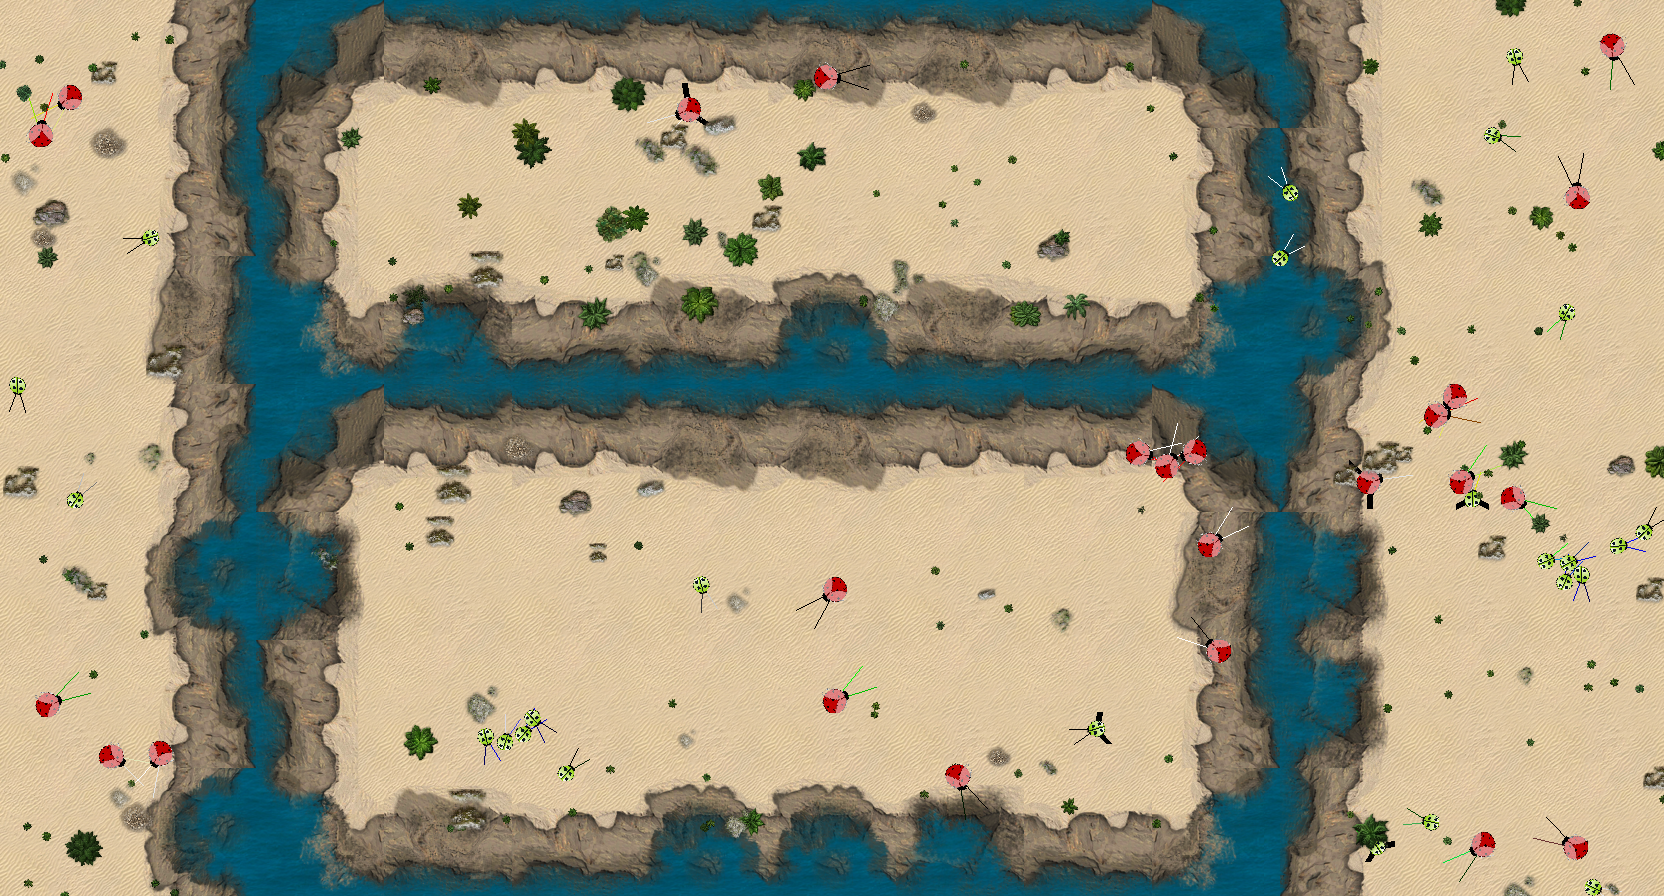
\includegraphics[width=0.8\columnwidth]{alife.png}
	\caption{\label{a_figure}An example figure}
\end{figure}


\section{Conclusion and Future Work}
	This section summarizes the paper: Your environment and agent, its strength and its weaknesses. Also remark about what would be the next steps you would take if you or someone else were to continue/extend this project. 
	Note that for the initial submission you are limited strictly to 4 pages (double column), \emph{not including references}. An extra page will be allowed for final submission (after the initial reviews). 

% The bibliography:
\begin{thebibliography}{4}

	\bibitem{Barber} % Book
	D.~Barber. Bayesian Reasoning and Machine Learning,
	{\em Cambridge University Press}, 2012.

	\bibitem{LectureSOP} % Web document
		J.~Read. Lecture III - Structured Output Prediction and Search. \textit{INF581 Advanced Topics in Artificial Intelligence}, 2018.

	\bibitem{Astar}
	D.~Mena et al. A family of admissible heuristics for A* to perform inference in probabilistic classifier chains.
	{\em Machine Learning}, vol. 106, no. 1, pp 143-169, 2017.

	\bibitem{DeepMindSC2}
	O.~Vinyals et al. StarCraft {II:} {A} New Challenge for Reinforcement Learning.
	\url{https://arxiv.org/abs/1708.04782}, 2017. 

\end{thebibliography}

% Your document ends here!
\end{document}
